\section{Attack Surface \& Models}
\todo[inline]{Link scenarios to CVSS}

Because Docker is more of an ecosystem than a single running process, it has quite a large attack surface. This attack surface consists of multiple attacker models.

\hfill

Lets take a look at the following images showing the attacker models.
We see the following processes pictured in the images.
\begin{enumerate}
    \item[A)] Standard (privileged) process running directly on the host.
    \item[B)] Standard unprivileged process running directly on the host.
    \item[C)] Process running in a Docker container.
    \item[D)] Similar to C.
\end{enumerate}

\subsubsection*{Container Escape}
\begin{figure}[ht]
    \centering
    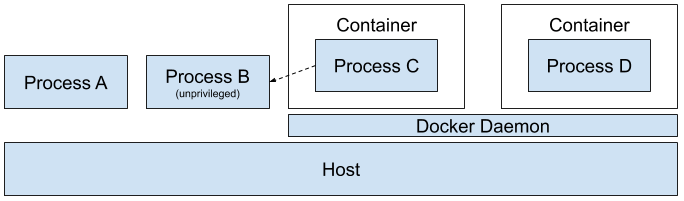
\includegraphics[width=.9\linewidth]{resources/images/attack-scenario-3.png}
    \caption{}\label{fig:container-escape}
    \medskip
    \small
    A process (Process C) running inside a container accessing data on the host (that it should not be able to access), in this case Process B.
\end{figure}

\subsubsection*{Docker Daemon Attack}
\begin{figure}[ht]
    \centering
    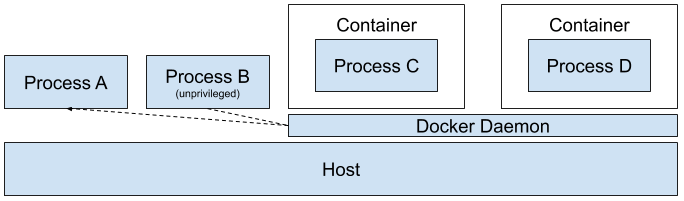
\includegraphics[width=.9\linewidth]{resources/images/attack-scenario-1.png}
    \caption{}\label{fig:docker-daemon-attack}
    \medskip
    \small
    An unprivileged process B accessing privileged data (in the image process A) using the Docker Daemon.
\end{figure}

\subsubsection*{Container Attack}
\begin{figure}[ht]
    \centering
    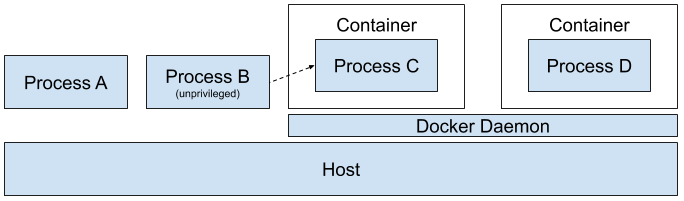
\includegraphics[width=.9\linewidth]{resources/images/attack-scenario-2.png}
    \caption{}\label{fig:container-attack}
    \medskip
    \small
    An unprivileged process B accessing data in a Docker container.
\end{figure}

\subsubsection*{Container to Container Attack}
\begin{figure}[ht]
    \centering
    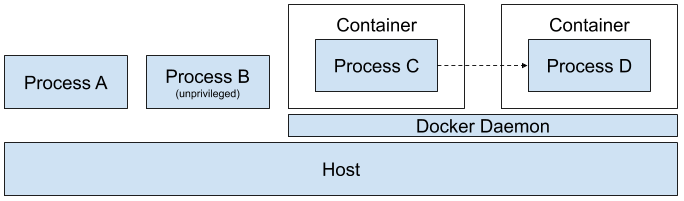
\includegraphics[width=.9\linewidth]{resources/images/attack-scenario-4.png}
    \caption{}\label{fig:container-to-container-attack}
    \medskip
    \small
    A process (Process C) running inside a container, accessing data in another container (process D).
\end{figure}

\subsection{Container Escape}
One of the most common type of vulnerability (and sometimes misconfiguration) is the possibility for a process running in a container to escape the container and access data (i.e.\ execute commands) on the host. This is shown in \autoref{fig:container-escape}.

\hfill

An example attack scenario would be a company that offers a PaaS (Platform as a Service) products that allows customers to run dockers on their infrastructure\footnote{This is actually quite common nowadays. All major computing providers offer such a service.}. If it is possible for the attacker to submit a Docker image that escapes the container and access the underlying infrastructure, they could access other containers or even other internal resources. That would, obviously, be a very big problem for that company.

\hfill

As noted before, because a container uses the same kernel and resources as the host; an exploit granting root can be just as devastating run inside as outside of the docker, because the target kernel and resources are the same.

It should also be noted that an exploit that allows someone to escape from a Linux \lstinline{namespace} is essentially a container escape exploit. CVE--2017--7308\cite{CVE-2017-7308} is a good example of this. Dirty Cow (CVE--2016--5195)\cite{CVE-2016-5195} is another good example of an exploit that allows container escapes\cite{Dirty-Cow-Escape}.

\subsection{Docker Daemon Attack \& Container Attack}
If user permissions are incorrectly configured, an unprivileged user can gain or access container resources they should not be able to access using the Docker Daemon. This is shown by \autoref{fig:docker-daemon-attack} and \autoref{fig:container-attack}.

\hfill

The Docker Daemon runs as \lstinline{root} (An experimental rootless mode is being worked on\footnote{\url{https://github.com/docker/engine/blob/master/docs/rootless.md}}). Because Docker has many (powerful) features, this allows any user with permissions to use Docker to practically gain \lstinline{root} privileges. This is why the Docker documentation explicitly states ``only trusted users should be allowed to control your Docker daemon''\cite{Docker-Daemon-Attack-Surface}

\hfill

A real life example of the impact of incorrectly configured Docker permissions happened a few years back with one of the courses in the Computing Science curriculum (of the Radboud). A teacher wanted to teach students about containerization and modern software development. He asked the IT department to install Docker on all student workstations and add all the students in the course to \lstinline{docker} group (giving them full permissions to run Docker). This gave every student the equivalent of \lstinline{root} rights on every workstation.

\subsection{Container to Container Attack}
Containers should not only be isolated from the host, but also from other containers. This allows multiple containers with sensitive data to be run on the same host without them being to access each other's data. In Docker this is not always the case. This is shown in \autoref{fig:container-to-container-attack}.

\hfill

By default all Docker containers are added to the same bridge network. This means that (by default) all Docker containers can reach each other over the network. This can lead to very dangerous situations. Lets say, for example, I run a database in a Docker container. I do not set a password for the database admin user, because I believe that the database is fully isolated (including the network) because of Docker. Any other Docker on that system is able to access the full database.


\subsection{Deployment \& Development Pipelines}
One of the biggest usages of Docker is automating part of the deployment and development process. Many developers use Continuous Integration and Deployment systems to automatically build Docker images that they then automatically pull and run on their production environments. This level of automation allows for very rapid software development.

That automation does have a negative side. It removes scrutiny from the deployment pipeline. If an attacker is able to compromise a link in the chain, they will be able to create their own malicious images that will be automatically run. Without proper monitoring of the full pipeline, such an attack can go unnoticed, because the system is designed to not need any human interaction.

\subsection{The impact of Docker on existing vulnerabilities}
A Docker container isolates software from the host, but does not change it. This means that vulnerabilities in software are not affected by Dockerizing that software. However, the impact of those vulnerabilities is decreased, because the vulnerability exists in an isolated environment.

If, for example, there exists a RCE (remote code execution) vulnerability in Wordpress. Running Wordpress in a Docker container does not fix the vulnerability. An attacker is still able to exploit it. But that attacker is not able to access the host system, because the exploited software is isolated from the host system because of Docker.

\subsection{Protection Mechanisms}
\todo[inline]{SELinux}
\todo[inline]{AppArmor}
\todo[inline]{Secure Computing Mode Profiles}
\todo[inline]{Capabilities}
\todo[inline]{\url{https://github.com/genuinetools/bane}}
\todo[inline]{CIS Benchmark Docker protections}
\todo[inline]{Docker Content Trust Signature Verification}
\todo[inline]{Wrapper scripts like docker-compose}
\todo[inline]{\url{https://docs.docker.com/engine/security/security/}}
